\documentclass[10pt]{beamer}

\usetheme{Montpellier}
\usecolortheme{beaver}

\usepackage{lmodern}
\usepackage{mathtools}
\usepackage{amsmath}
\usepackage{listings}
\usepackage{mdframed}
\usepackage{xcolor}
\usepackage{parskip}
\usepackage{substr}
\usepackage{hyperref}
\usepackage{etoolbox}
\usepackage{tipa}
\usepackage{pdfpages}
\usepackage{multicol}
\usepackage{cprotect}
\usepackage{booktabs}
\usepackage{silence}
\usepackage[backend=biber, style=ieee]{biblatex}
\usepackage[english,ngerman]{babel}
\usepackage{csquotes}
%\hypersetup{colorlinks = true, urlcolor=blue, linkcolor=white}
\mode<presentation>{}
\beamertemplatenavigationsymbolsempty
\setbeamertemplate{footline}[frame number]
\setbeamercolor{title in head/foot}{fg=black}
\setbeamercolor{subsection in head/foot}{fg=black}



\WarningFilter{biblatex}{Patching footnotes failed}

\renewcommand*{\bibfont}{\tiny}

\bibliography{resources.bib}

\titlegraphic{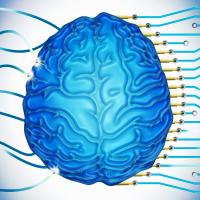
\includegraphics[keepaspectratio, height=0.1\textheight, width=0.5\textwidth]{img/logo_nmti.jpg} \\ [1em]
\includegraphics[keepaspectratio, height=0.07\textheight, width=0.5\textwidth]{img/logo_klinik.png} \\ [1em] 
\includegraphics[keepaspectratio, height=0.15\textheight, width=0.5\textwidth]{img/logo.png}}

\title{\textbf{Data-driven biomarkers for motor Subthalamic Nc. in PD during DBS electrode implantation}}
\author{\vspace{-0.7cm}F. Klopfer}
\date{\today}


\begin{document}
\frame{\titlepage}

\section{Introduction}
\begin{frame}
\begin{center}
 \begin{Huge}
  \textbf{Introduction}
 \end{Huge}
 \end{center}
\end{frame}
\subsection{}
%\subsectionpage
\begin{frame}[fragile]{Parkinson's Disease: Symptoms}
  as in 2023 ICD-10-CM Diagnosis Code G20: Parkinsonism~\autocite{who} \\ [2em]
    \begin{itemize}
     \item progressive motor disability: tremors, shaking, muscular rigidity, stiffness, slowing of movements, and lack of postural reflexes. \\ [2em]
     \item Non-motor symptoms: Slurrish speach, sleeping problems, depression, anxeiety
    \end{itemize}
     \framebreak
     \end{frame}


\begin{frame}[fragile]{Parkinson's Disease: Assessment}
     e.g. with MDS-UPDRS~\autocite{mdsupdrs}\footnote[frame]{Movement Disorder Society Unified Parkinson's Disease Rating Scale} consisting of 4 parts:
      \begin{enumerate}[I.]
        \item Nonmotor aspects of daily living: Cognitive impairments, mood, depression \& anxiety, sleep problems, pain, $\dots$
        \item Motor aspects: Speech, eating, dressing, hygiene, handwriting $\dots$
        \item Motor examination by clinicean (Speech, facial expressions, rigidity, hand movements, $\dots$) with/out medication with L-DOPA
        \item treatment-related motor complications: fluctuations and dyskinesia \\ [2em]
      \end{enumerate}
      Also possible: SPECT for DA transporters\footnote[frame]{Single Photon Emission Computed Tomography}
    \end{frame}

\begin{frame}[allowframebreaks, fragile]{Parkinson's Disease: Mechanisms}
      \begin{itemize}
        \item loss of dopamine-producing/melanin-containing neurons in substantia nigra pars compacta~\autocite{mechanisms}
        \item accumulation of lewy bodies in SN and VTA~\autocite{syn} among others
        \item Reason unknown; Combination of genetic and environmental factors hypothesized~\autocite{pink, mechanisms}
      \end{itemize}
      \framebreak
    \begin{multicols}{2}
    \begin{minipage}{0.49\textwidth}
     \includegraphics[keepaspectratio,width=0.8\textwidth,height=0.8\textheight]{img/0.jpg}
    \end{minipage} \vfill \null
    \begin{minipage}{0.49\textwidth}
     \begin{itemize}
      \item Degradation of nigrostriatal DA pathway \\ [2em]
      \item impairs regulation of Basal Ganglia circuit \\ [2em]
      \item greater inhibition of voluntary movements \\ [2em]
     \end{itemize}
    \end{minipage}
    \end{multicols}


    \framebreak
    \begin{center}
    \includegraphics[keepaspectratio,width=0.95\textwidth,height=0.95\textheight]{img/1.png}
     \end{center}
     \end{frame}

 \begin{frame}[allowframebreaks, fragile]{Parkinson's Disease: DBS~\autocite{ghara}}
  \begin{center}
   \includegraphics[keepaspectratio,width=0.8\textwidth,height=0.8\textheight]{img/2.png}
  \end{center}
  \framebreak
      \begin{multicols}{2}
    \begin{minipage}{0.49\textwidth}
      \includegraphics[keepaspectratio,width=0.9\textwidth,height=0.9\textheight]{img/2_1.png}
         \end{minipage} \vfill \null
    \begin{minipage}{0.49\textwidth}
Stimulation with high frequency to inhibit target structure

    \end{minipage}
    \end{multicols}
\end{frame}

\begin{frame}[allowframebreaks, fragile]{Data}
   \begin{center}
    \includegraphics[keepaspectratio,width=\textwidth,height=\textheight]{img/dataset.png}
    \end{center}
\framebreak
  \begin{itemize}
   \item Pre-Operative:
   \begin{itemize}
    \item Imaging: CT, MRT (incl. DTI)
    \item Questionaires: MDS-UPDRS, PDQ39, BDI, MoCA
   \end{itemize}
   \item Intra-Operative:
      \begin{itemize}
       \item (Bio-)Signals: EEG, Micro-electrode recordings, DBS electrode recordings
       \item Imaging: CT/Angiography
      \end{itemize}

   \item Post-Operative:
      \begin{itemize}
        \item Imaging: CT, MRT
        \item Questionaires: as above
        \item (Future Work: Wearables, Sleep EEG)
      \end{itemize}
  \end{itemize}
\end{frame}

\begin{frame}[allowframebreaks, fragile]{Surgery}
  \begin{enumerate}
   \item Plan implantation stereotactically using CT and MRT.
   \item [...]
   \item Fixate stereotactic frame \& EEG on patient.
   \item [...]
   \item First trajectroy with micro-electrode to quantify activity (spiking).
   \item Then with Deep Brain Stimulation electrode (e.g. Abott St. Jude 6172) milimeterwise, measuring at each position for 30s \& calculate PSD. Implant according to patient profile.
   \item [...]
   \item continue with other side.
   \item End surgery for DBS lead implantation, continue with generator and cable.
  \end{enumerate}
  \framebreak
  \begin{center}
   \includegraphics[keepaspectratio, width=0.9\textwidth, height=0.49\textheight]{img/mapping.png}
  \end{center}
  \begin{center}
   \includegraphics[keepaspectratio, width=0.9\textwidth, height=0.49\textheight]{img/circuits.png}
  \end{center}
\end{frame}

\section{Task \& Approach}
\begin{frame}
\begin{center}
 \begin{Huge}
  \textbf{Task \& Approach}
 \end{Huge}
 \end{center}
\end{frame}

\begin{frame}{Task}
  \begin{itemize}
   \item[Given:] A set of potiential biomarkers/features. \\ [3em]
   \item[Desired:] Framework for quantifying the quality of (combinations of) biomarkers/features. \\ [3em]
   \item[Ansatz:] Apply classification to predict and Shapley values~\autocite{shap1} to assess feature importance.
  \end{itemize}
\end{frame}

\begin{frame}{Shapley Values}
Roots in game theory~\autocite{shapley1953value}
\begin{itemize}
 \item Coalition of players obtaining overall gain from cooperation \\ [1em]
 \item Shapley values answer the questions: How important is each player to the coalition overall? What payoff can they expect? \\
 \end{itemize}
 Transfer~\autocite{shap}
 \begin{itemize}
 \item Coalition = set of features. Player = single feature. \\ [2em]
 \item How important was one feature to the prediction (using the set of features) overall?
\end{itemize}
\end{frame}

\begin{frame}{Application}
  \begin{itemize}
   \item[Given:] Signals recorded during surgery \\ [3em]
   \item[Desired:] What are electrophysiological biomarkers of motor part of STN? \\ [3em]
   \item[Ansatz:] Use Classification to predict if DBS electrode is inside/outside of motor STN and Shapley values~\autocite{shap1} to assess feature importance
  \end{itemize}
\end{frame}


\begin{frame}[allowframebreaks, fragile]{Setup}
\begin{itemize}
 \item Use normalized\footnote[frame]{Fit the spectrum with FOOOF and subtract the aperiodic part} PSD binned by 5 Hz \\ [1em]
 \item Use simple classifier: DecisionTree from sklearn\\ [1em]
 \item Electrode position gathered from reconstruction\\ [3em]
\end{itemize}
\begin{tabular}{l l l l l} \toprule
patients & samples & depth range & recording time & in motor STN \\ \midrule
42 & 5122 & $[10, 20]$ mm & $42.68\overline{3}$ hours & 1052 \\
\bottomrule
\end{tabular}
\framebreak
  \begin{center}
  \includegraphics[keepaspectratio,width=0.95\textwidth,height=0.95\textheight]{img/coreg.png}
    \end{center}
    \framebreak

\end{frame}
\begin{frame}[allowframebreaks,fragile]{Results}
  \begin{center}
  \includegraphics[keepaspectratio,width=0.95\textwidth,height=0.95\textheight]{img/DecisionTree_shap_bar.png}
    \end{center}
    \framebreak

  \begin{center}
  \includegraphics[keepaspectratio,width=0.95\textwidth,height=0.95\textheight]{img/DecisionTree_shap_beeswarm.png}
    \end{center}
\end{frame}



\section{Outlook}
\begin{frame}
\begin{center}
 \begin{Huge}
  \textbf{Outlook}
 \end{Huge}
 \end{center}
\end{frame}

\begin{frame}{Outlook}
\begin{itemize}
 \item Extend PSD frequency range
 \item additional types of features (e.g. median absolute deivation)
 \item other means than mean absolute shap value!
 \item within STN classification (motor, associative, limbic), STN vs SN, ...
 \item Use features with highest shap value to cluster/reclassify
 \item more complex classifier (e.g. those applying transformations)
 \item multi-label classification
\end{itemize}
\end{frame}


\section{Institute for Neuromodulation \& -technology}
\begin{frame}
\begin{center}
 \begin{Huge}
  \textbf{Institute for Neuromodulation \& -technology} \\
 \end{Huge}
 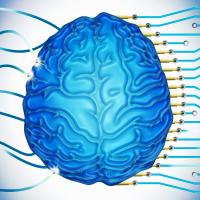
\includegraphics[keepaspectratio, height=0.4\textheight, width=0.5\textwidth]{img/logo_nmti.jpg}
 \end{center}
\end{frame}

\begin{frame}{Overview}
\begin{itemize}
  \item Stimulating \& Recording:
  \begin{itemize}
  \item Non-invasive: tACS, tDCS, tMS, VNS + EEG
  \item Invasive: MER, DBS, (VNS) \hfill \textbf{in-vivo intracranial subcortical data!}
  \end{itemize}
  \item Diseases:
  \begin{itemize}
   \item Parkinson's disease
   \item Stroke
   \item Motor deficits
   \item Some brain tumors, some epilepsy
  \end{itemize}
  \item Other topics: sleep, plasticity, surgical methods
\end{itemize}
\end{frame}

\begin{frame}
 \begin{center}
  \includegraphics[keepaspectratio, width=\textwidth, height=\textheight]{img/surgery.jpg}
 \end{center}

\end{frame}

     
\section{References}
    \begin{frame}[allowframebreaks]
      \frametitle{References}
      \begin{tiny}
      \nocite{*}
      \printbibliography
      \end{tiny}
    \end{frame}

\appendix
\section{Appendix}
\begin{frame}[allowframebreaks, fragile]{Pre-, Intra- and Post-OP CT}
     \begin{center}
    \includegraphics[keepaspectratio,width=0.7\textwidth,height=0.7\textheight]{img/pre_ct.png}
     \end{center}
     \framebreak

      \begin{center}
    \includegraphics[keepaspectratio,width=0.7\textwidth,height=0.7\textheight]{img/inop_ct.png}
     \end{center}
     \framebreak

      \begin{center}
    \includegraphics[keepaspectratio,width=0.7\textwidth,height=0.7\textheight]{img/inop_ct_arti.png}
    \end{center}
    \framebreak

    \begin{center}
    \includegraphics[keepaspectratio,width=0.7\textwidth,height=0.7\textheight]{img/angio.png}
    \end{center}
    \framebreak

      \begin{center}
    \includegraphics[keepaspectratio,width=0.7\textwidth,height=0.7\textheight]{img/post_ct.png}
     \end{center}
\end{frame}



 \end{document}
